% \textcolor{red}{(The Introduction chapter should contain background information as appropriate, plus definitions of all special and general terms. Your topic should be: clearly stated and defined; have a clear overall purpose; and have clear, relevant and coherent aims and objectives. It is also informative to give a brief description of the contents of the remaining chapters of the thesis. This alerts the reader and prepares them for the rest of the thesis.)}

% \colin{Physics motivation and MSSM should not be part of Introduction. Call this chapter: Physics motivation. Then you need to talk about the standard model, the higgs, the mssm, etc. }

% \colin{example of use of the ptdr macros:}

% $\pt = 150\,\pbinv$

% particle flow~\cite{CMS-PRF-14-001}

The theoretical context of this research is presented in the following chapter. The Standard Model, introduced in section \ref{sec:SM}, is the widely accepted basis of particle physics understanding. Its Higgs sector will be focused on in section \ref{sec:SM_higgs}. But the Standard Model has several limitations, which will be discussed in section \ref{sec:SM_limits}. One of the promising extension of the standard model, called the Minimal Supersymetric extension of the Standard Model (MSSM) will then be described in section \ref{sec:MSSM}. Finally the phenomenology of the detection of the Higgs sector of the MSSM in proton-proton collisions will be presented in section \ref{sec:pheno}.

\section{Overview of the Standard Model}
\label{sec:SM}
The Standard Model (SM) is the prevalent theoretical framework that describes fundamental elements, named particles, and their interactions. As a quantum field theory, this framework considers particles as excited states of fundamental quantum fields. The interactions between these particles are the forces of nature : electromagnetic, weak and strong. Gravity is not included in the SM as it hasn't been successfully described by a quantized interaction that complies with general relativity. The SM also lacks explanation for several phenomena of nature, and is therefore considered incomplete. But its validity is not questioned as it has provided confirmed predictions and has not been successfully contradicted by a particle physics experiment yet. An overview of the standard model content in term of particles and their characteristics is shown in Figure \ref{fig:SM}.\newline

\begin{figure}
    \centering
    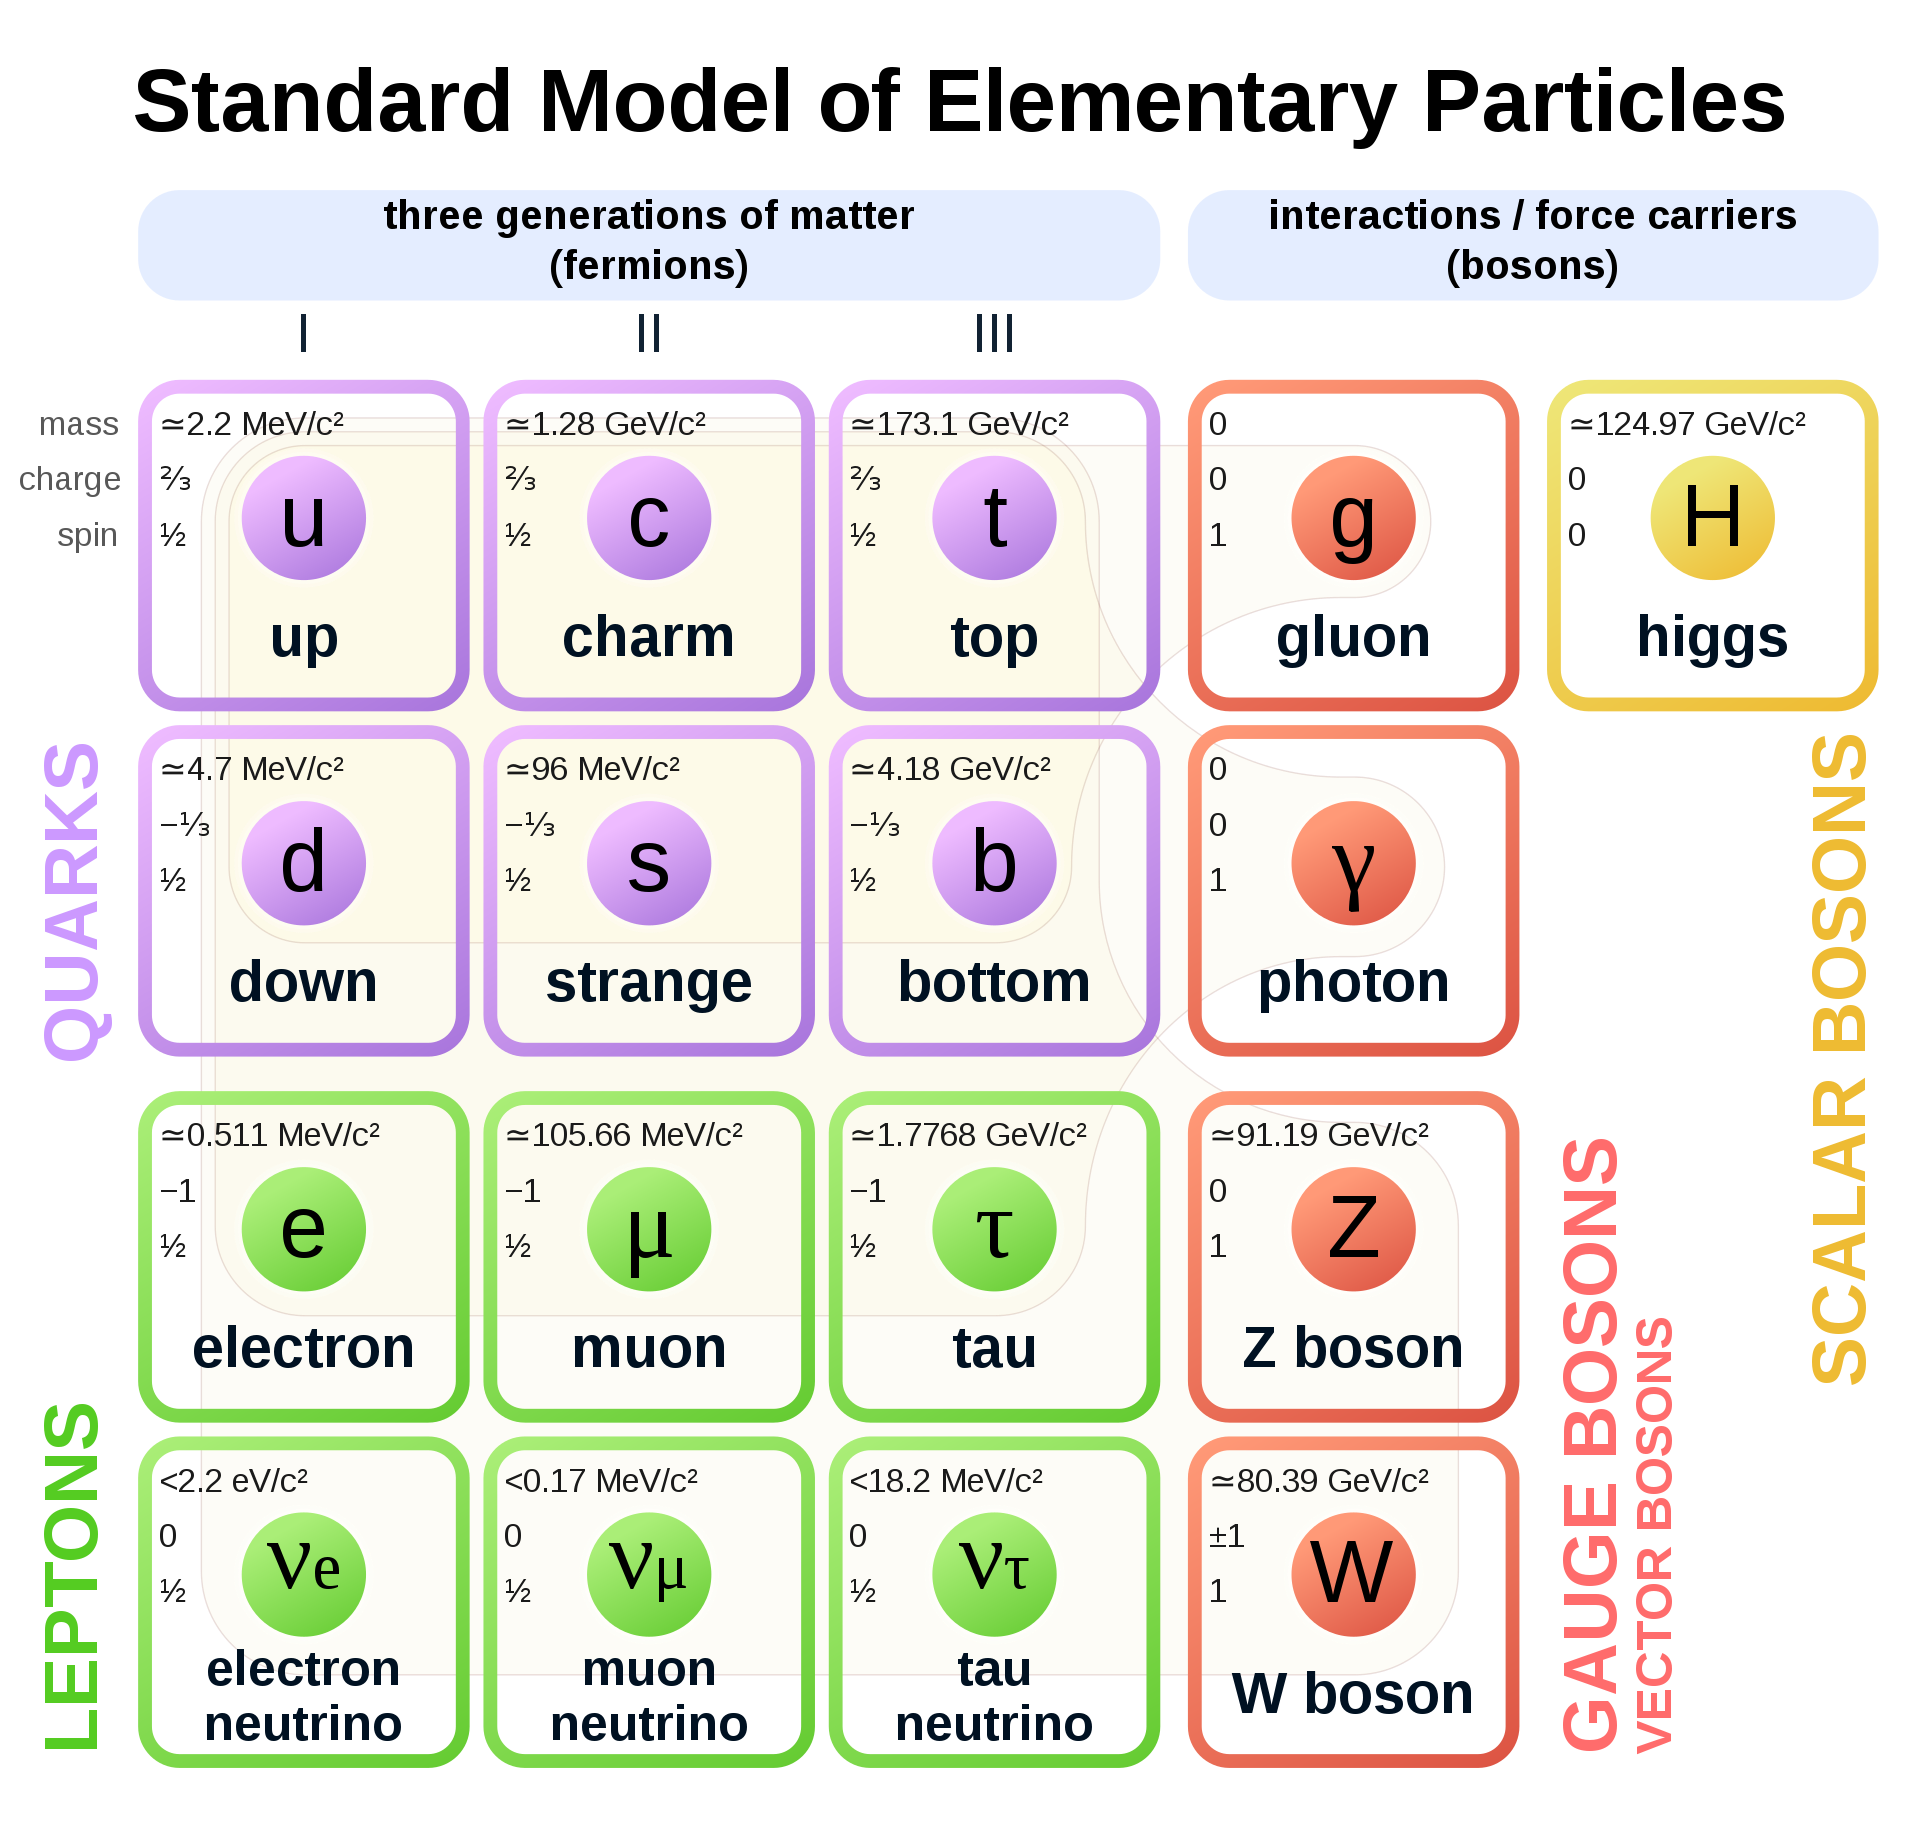
\includegraphics[width=0.7\textwidth]{Images/SM_zoo.png}
    \caption{Overview of the standard model content in term of particles and their characteristics from \cite{SMschema}.}
    \label{fig:SM}
\end{figure}

Mathematically, the SM is described by a non-abelian gauge quantum field theory. A gauge theory is a type of field theory whose equations of motion are invariant under a continuous group of local transformations of the fields which can be written $\psi \rightarrow \psi' = e^{i\lambda(x)}\psi$. The SM contains internal symmetries of the Lie's algebra unitary product group $SU(3)_C \times SU(2)_L \times U(1)_Y$, corresponding to the strong and electroweak forces. However, the electroweak symmetry is broken at low energies, and therefore the internal symmetries effectively become $SU(3)_C \times U(1)_Q$ in which the first term represent the strong and the second the electromagnetic symmetry.

The SM is conventionally expressed using the lagrangian formalism. From this formalism, the principle of least action is equivalent to \cite{Thomson:2013zua}
\begin{equation}
    \delta \mathcal{S} = \int \mathrm{L} dt = \int \Lagr(\phi,\partial_{\mu}\phi) d^4 x = 0 \mend
    \label{eq:lagr_density}
\end{equation}

In this equation, $\phi$ represents a field and $\partial_{\mu}$ represent the space and time derivatives following Einstein's notation. The integration over all the space of the lagrangian density $\Lagr$ in equation \ref{eq:lagr_density} is by convention usually implicit and the formulation of future lagrangian terms will be given in terms of lagrangian density.

Observable particles are considered to be excited states of the fundamental fields. Two types of fields, and therefore of particles, can be differentiated in the lagrangian terms by one defining property : the spin. Historically, this property allows particles to react to the presence of a magnetic field, in a sort of intrinsic angular momentum. The spin-statistics theorem allows then to classify particles into two types : the fermions, with half-integer valued spins, and the bosons with integer valued spins. Fermions are effectively the constituents of matter while bosons are the carriers of the different forces.

\subsection{Fermions}

Fermions ($\psi$) are the fundamental particles that compose matter. They are described mathematically by the Fermi-Dirac statistics, which means that their spin has a half-integer value and therefore obey the Pauli exclusion principle and the canonical anti-commutation relations.

In the following equations, the convention $c = \hbar = 1$ is used, and will be used throughout this thesis. The notation $\slashed{\partial} = \gamma^{\mu}\partial_{\mu}$ is also used and the $\gamma^{\mu}$ matrices are defined in appendix \ref{appendixA}. \newline

In order to keep the Lorentz invariance, a hermitian conjugate of the fermionic field has to be defined such as $\Bar{\psi} \equiv \psi^{\dagger}\gamma^0$, which will then represent the antimatter particles, which has the same characteristics but opposite quantum numbers.\newline

The fermionic term of the lagrangian can be written, for all fermionic fields :

\begin{equation}
    \Lagr_f = i\Bar{\psi}\slashed{\partial}\psi - m\Bar{\psi}\psi \mend
    \label{eq:free_fermion}
\end{equation}

The fermionic field takes then the form of a plane wave 

\begin{equation}
    \psi(x) = \int \frac{d^3 p}{(2\pi)^3} \frac{1}{\sqrt{2E_p}} \sum^{2}_{s} \Big( a^{s}_{P} u_s (p)e^{-ipx} + b^{s\dagger}_P v_s (p)e^{ipx} \Big) \mend
\end{equation}
In this equation, $u_s (p)$ and $v_s (p)$ are spinors with momentum p and spin s; $a^{s}_P$ and $b^{s\dagger}_P$ are the creation and annihilation operators respectively, which act as a base for the Fourier transform of the field. The creation operator raises the field level, creating new excited states. On the other hand the annihilation operator de-excites the field.

The terms in equation \ref{eq:free_fermion} can also be rewritten such as to separate the fermions in their chiral components, as it is useful in cases where interactions are sensitive to chirality. The chiral operator $\gamma^5 \equiv i\gamma^0 \gamma^1 \gamma^2 \gamma^3$ is used to write
\begin{equation}
    \psi = \frac{1- \gamma^5}{2}\psi + \frac{1+ \gamma^5}{2}\psi = P_L \psi + P_R \psi = \psi_L + \psi_R \mend
\end{equation}

The orthogonality of the components leads to the mass term of equation \ref{eq:free_fermion} to become

\begin{equation}
    \Bar{\psi}\psi = (\Bar{\psi}_R + \Bar{\psi}_L)(\psi_L + \psi_R) = \Bar{\psi}_R \psi_L + \Bar{\psi}_L \psi_R \mend
    \label{eq:chiral_fermions}
\end{equation}

The fermions of the SM can be split into two categories, namely the quarks and the leptons. The main difference is the fact that the quarks carry colour charges, making them susceptible to interactions through the strong force. Also, leptons carry an integer electric charges whereas quarks carry electric charges of either $1/3$ or $2/3$.

Both quarks and leptons can be classified into three generations depending on their mass. The first generation contains the most commonly encountered particles in our world, and the two other generations contains particles with the same characteristics, except higher masses. So far only three generations are known and the possibility of other generations is constrained by the Z boson decay \cite{2006257}, although the validity of this affirmation depends on the mass and couplings of the neutrinos with the Z boson.

\subsubsection{Quarks}

Quarks ($\psi_q$) are by definition fermions that carry a colour charge. Colour is the strong force charge, and has three distinct types, namely red, green and blue. Anti-quarks have opposite quantum numbers, therefore they carry charges one of anti-red, anti-green or anti-blue. In each generation there are two types of quarks as weak isospin doublets, the up-type and the down-type, leading to 3 doublets. The up-type quarks are the up (u), charm (c) and top (t) and have an electric charge of $+\frac{2}{3}$. Their weak isospin partners, the down-type quarks are named down (d), strange (s) and bottom (d) and have an electric charge of $-\frac{1}{3}$.

Because they carry a colour charge, quarks are subjected to confinement, a consequence of the nature of the strong interaction, which will be detailed in section \ref{sec:QCD}. Indeed, in nature quarks are only observed combined into composite particles holding neutral color charge (white), called hadrons. Usual hadrons are mesons and hadrons. Mesons are hadrons composed of a quark and an anti-quark with opposite colours (e.g. red and anti-red). Baryons are composed of three quarks of different colours, making them colour-neutral as a whole. Mesons have integer spin value, meaning they will behave effectively as bosons, whereas baryons have a half-integer value, behaving effectively as fermions. Ordinary matter nuclei are composed of proton and neutron, which are baryons of composition ($uud$) and ($udd$) respectively.

\subsubsection{Leptons}

Leptons ($\psi_l$) are fermions but contrarily to quarks, they do not have a color charge, and therefore are not sensitive to the strong force. In a similar way to the quarks being ordered in three generations of weak isospin doublets, leptons can be split into doublets of an electron-like and a neutrino. The electron-like group is composed of the electron (e), the muon ($\mu$) and the tau lepton ($\tau$), each of which has an electric charge of $-1$ ($+1$ for their antiparticles), thus they interact through the weak and electromagnetic forces. On the other hand the neutrino group is composed of electrically neutral particles, meaning they only interact through the weak force. Neutrinos are named from their weak isospin partners: electron neutrino ($\nu_e$), muon neutrino ($\nu_{\mu}$) and tau neutrino ($\nu_{\tau}$). They have been proven to be massive, but their mass is so low that it is considered negligeable in accelerators experiments. In addition, they only interact through the weak force, making neutrinos elusive particles and hard to detect in practice.

\subsection{Bosons}

To conserve gauge invariance, equation \ref{eq:free_fermion} should not be changed by an infinitesimal rotation of the fermionic field of the form $e^{i\lambda(x)}$. The Noether theorem states that every symmetry implies a conserved quantity. In the case of the electromagnetic interaction (QED), this leads to

\begin{equation}
    \partial_{\mu}j^{\mu} = \partial_{\mu}(-e\Bar{\psi}\gamma^{\mu}\psi) = 0 \mend
\end{equation}
The current $j^{\mu}$ is then conserved, and so is the associated charge $Q = \int j^{0}d^3 x$.

The fermionic fields transforms as
\begin{equation}
    \psi \rightarrow \psi' = e^{i\lambda(x)Q}\psi \mend
\end{equation}
However, the standard derivative do not conserve the invariance for these rotations since
\begin{equation}
    \partial_{\mu}\psi \rightarrow \partial_{\mu}\psi' = e^{i\lambda(x)}\partial_{\mu}\psi + iQe^{i\lamdda(x)}\psi\partial_{\mu}\lambda(x) \mend
\end{equation}
To recover gauge invariance, the covariant derivative must be introduced:
\begin{equation}
    D_{\mu}\psi \rightarrow e^{i\lambda(x)Q}D_{\mu}\psi \mend
\end{equation}
To be able to write such a derivative, the field $A_{\mu}$ must be introduced such as
\begin{equation}
    D_{\mu} = \partial_{\mu} + ieQA_{\mu}
\end{equation}
where $A_{\mu}$ transforms as
\begin{equation}
    A_{\mu} \rightarrow A_{\mu} - \frac{1}{e}\partial_{\mu}\lambda(x) \mend
\end{equation}
The $A_{\mu}$ field can be associated with the photon in this case.
Indeed, the Yang-Mills theory \cite{PhysRev.96.191} is a non-abelian gauge field theory based on the internal continuous symmetries, the special unitary group $SU(N)$, of the Lie algebra. The $SU(N)$ is a symmetry group of $N \times N$ unitary matrices with determinant 1 and $N^2 -1$ generators. The generators are then the different bosons associated with each field.
More generally, bosons are excited states of the fields associated with the fundamental forces in the SM. They are effectively considered carriers or mediators for these fundamental forces. The forces in question are first the strong interaction, responsible for nuclear cohesion, and second the electroweak force (EW), which actually breaks down into two different interaction at low energies : the electromagnetic and the weak interactions.
Mathematically, bosons have to obey the canonical commutation relations and they follow the Bose-Einstein statistics, which means their spin value is of integer value.

The bosonic fields contribute several terms in the lagrangian corresponding to the free propagation, the self-interaction and the interaction with other fields. The free propagation and the self-interaction terms are usually combined into a kinematic term

\begin{equation}
    \Lagr_{kin} = -\frac{1}{4}F^{a}_{\mu\nu}F_{a}^{\mu\nu} \msep
\end{equation}
where
\begin{equation}
    F^{a}_{\mu\nu} \equiv \partial_{\mu}A_{\nu}^a - \partial_{\nu}A_{\mu}^a + g f_{bc}^a A_{\mu}^b A_{\nu}^c \mend
\end{equation}
In this expression, $g$ is the coupling constant, a parameter associated with the relative strength of the force, and $f_{bc}^a$ is the structure constant. This structure constant is defined in a Lie algebra from the commutator of two generators of the group as
\begin{equation}
    \big[ T_a , T_b \big] = i f_{bc}^a T_c \mend
    \label{eq:commut}
\end{equation}
The two fundamental forces of the SM are the strong force and the electroweak interaction and are described through similar bosonic fields, with an associated set of fundamental bosons.

\subsection{Quantum Chromodynamics}
\label{sec:QCD}

In the Standard Model, the quantum field theory associated with the strong force is called Quantum Chromodynamics (QCD), as the conserved charge linked with this interaction is named colour. Colour was theorized from the discovery in 1951 of the $\Delta^{++}$ baryon. Indeed this baryon is composed of three up quarks ($uuu$). This baryon's spin is $\frac{3}{2}$ and up quarks are fermions of spin $\frac{1}{2}$. This would therefore lead to the conclusion that these up quarks are in the exact same quantum state, contradicting Pauli's exclusion principle. Indeed, considering this new charge, all three quarks would each carry a different color charge, avoiding Pauli's exclusion principle. Mesons and baryons are then colour-neutral, which is confirmed by observations.

QCD is a non-abelian Yang-Mills gauge theory that corresponds to the $SU(3)_C$ sector of the SM. The bosonic field $G_{\mu}^a$ is called gluon field. To express the free term of the interaction, the strength tensor field $G_{\mu\nu}^a$ is defined as

\begin{equation}
    G_{\mu\nu}^a \equiv \partial_{\mu}G_{\nu}^a - \partial_{\nu}G_{\mu}^a + g_{s}f_{bc}^{a}G_{\mu}^{b}G_{\nu}^{c} \mend
\end{equation}
In this expression, the index $a$ refers to the color charge, $g_s$ is the strong coupling constant, and $f_{bc}^a$ is the result of the commutator of the generators of the group as described in equation \ref{eq:commut}. In the SU(3) group symmetry, there are eight different generators, meaning eight gluons, that mathematically take the form of the Gell-Mann matrices divided by two, as detailed in appendix \ref{appendixA}.

The color-triplet of fermions and its derivative transform under the SU(3) group as
\begin{equation}
    \partial_{\mu}\psi_Q \rightarrow \partial_{\mu} \psi_{Q}' = \partial_{\mu}\psi_Q + ig_s T_a G_{\mu}^a
\end{equation}
leading to the covariant derivative
\begin{equation}
    \partial_{\mu} \rightarrow D_{\mu} \equiv \partial_{\mu} - ig_s T_a G_{\mu}^a \mend
\end{equation}

Finally, by combining the kinematic term for both quarks and gluons to the interaction term of QCD leads to :

\begin{equation}
    \Lagr_{QCD} = i\Bar{\psi_Q} (\slashed{D}_{\mu} - m ) \psi_Q - \frac{1}{4} G_{\mu\nu}^a G^{\mu\nu}^a
\end{equation}

Important specific properties of the QCD interaction are asymptotic freedom and confinement. Asymptotic freedom is the fact that QCD interaction grows weaker as the energy increases or distance decreases. This makes the quarks and gluons inside hadrons effectively free particles for short range interactions. On the other hand confinement is a postulate of QCD driven by observations, stating that color-charged particles cannot exist isolated in nature. In effect only color-neutral composite particles can be stable, separating them would lead the QCD potential energy to rapidly grow and create pairs of quark-antiquark. The newly created quarks will then start associating and creating new pairs of quarks until only color-neutral hadrons are left. This process happens when quarks are created in high energy collisions such as at the LHC, and is called hadronization.

\subsection{The electroweak theory}

At low energies, two additional forces are known : the electromagnetic and weak interactions. The electromagnetic force is an infinite-range interaction responsible for the cohesion of atoms, where the weak force is historically the interaction responsible for various nuclear decays. In the early developments of particle physics, both forces were described as independent interactions, as these forces manifest themselves in very different ways. At the time the weak force was known as Fermi's interaction \cite{Fermi2008}, a mechanism describing the interaction of four fermions as a point-like process, as shown in Figure \ref{fig:fermi_int}.

The electromagnetic force was successfully quantized by Schwinger, Tomonaga, Feynman and Dyso, leading to the birth of Quantum Electrodynamics (QED) \cite{PhysRev.80.440,PhysRev.76.749,PhysRev.76.769,PhysRev.74.1439,PhysRev.73.416,10.1143/PTP.1.27} . It was described as an interaction of two fermions with the mediation of a boson, the photon ($\gamma$). QED was gauge invariant and overall renormalizable. These features pushed the physics community to consider gauge symmetries as fundamental symmetries of nature, and to try to formalize the other forces in the context of a gauge theory. However, these attempts failed due to the weak interaction's short range and the fact that it was not renormalizable.

To overcome this, Schwinger proposed a description of the weak interaction analogue to the one of the electromagnetic force \cite{SCHWINGER1957407}. The weak force would not be a short-range interaction of 4 fermions but a long-range interaction of two fermions mediated by a charged vector boson, called $W^{\pm}$ \ref{fig:melectroweak}. The similarities between QED and this weak force, and the root of the gauge invariance, led to the hope of unification of the two forces. Many attempts were done in the following years with little success, though small advances were achieved. One such advance was parity (P-symmetry) violation, meaning a behavioral difference of chiral components. This could be achieved by a Vector-Axial theory (V-A theory) \cite{PhysRev.109.193,PhysRev.109.1860.2}, in which QED would play the vectorial role.

\begin{figure}
\centering
\begin{subfigure}[b]{0.5\textwidth}
  \centering
  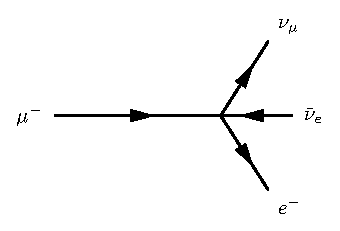
\includegraphics[width=\textwidth]{Images/fermi1.pdf}
  \caption{\label{fig:fermi_int}}
\end{subfigure}%
\begin{subfigure}[b]{0.5\textwidth}
  \centering
  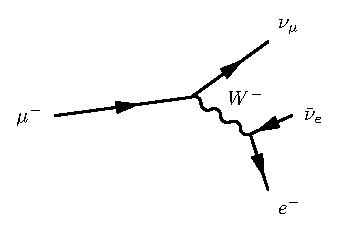
\includegraphics[width=\textwidth]{Images/fermi2.pdf}
  \caption{\label{fig:melectroweak}}
\end{subfigure}
\caption{Feynman diagrams for the muon decay as (\subref{fig:fermi_int}) a Fermi's interaction, without a propagator and (\subref{fig:melectroweak}) a Yang-Mills theory mediated by a $\mathrm{W}^{-}$ boson.}
\label{fig:etomununu}
\end{figure}

In 1961, Sheldon Glashow proposed a $SU(2) \times U(1)$ Yang-Mills theory \cite{GLASHOW1961579} to unify both interaction.  The proposal defined two fields, $B_{\mu}$ and $W_{\mu}^a$, with four fundamental bosons, $B$ and $W^i$. The observable features, like the vector bosons $W^{\pm}$ and $Z$, were actually a linear combination of both fields with a mixing angle called $\theta_W$. But the model had several flaws and was ignored at the time.

First, it predicted a new phenomena for which there was no evidence at the time: neutral conserving-flavor currents, mediated by a neutral massive vector boson different from the photon. Second, its renormalizability was unclear. Finally, the experimental results had only evidence that the interaction was extremely short-ranged, pushing towards the existence of a massive, charged weak boson. But chiral Yang-Mills theories, being gauge invariant, did not allow the addition of a mass term.

The solution actually came from the field of condensed matter. Work on superconductivity led to the establishment of the Goldstone theorem \cite{PhysRev.127.965}, which states that scalar bosons, named Goldstone bosons, arise from the breaking of global continuous symmetries. However, the predicted bosons were not always observed. The models trying to employ the spontaneous symmetry breaking (SSB) encountered the same problem.

Philip Anderson pointed out in 1963 \cite{PhysRev.130.439} that in a degenerated state within a gauge potential, the massless Goldstone bosons could combine with the massless propagators of the gauge field to become massive bosons. The Goldstone bosons would therefore not appear as observables and the massless vector bosons of the theory would acquire a mass, solving both issues. Indeed in superconductivity this phenomenon appears when photons interact with the electromagnetic potential in a superconducting electron gas : massless photons become massive plasmons, and no Goldstone boson appears.

In the summer of 1964, three groups of physicist developed independently such a mechanism based on SSB to give mass to gauge bosons in the QFT framework by adding a new scalar field : François Englert and Robert Brout in August 1964 \cite{PhysRevLett.13.321}, Peter Higgs in October 1964 \cite{HIGGS1964132,PhysRevLett.13.508} and Gerald Guralnik, Carl Hagen and Tom Kibble in November 1964 \cite{PhysRevLett.13.585}. This was the birth of the Brout-Englert-Higgs mechanism, more commonly known as the Higgs mechanism. Peter Higgs was the only one to remark explicitly a consequence of the addition of the new scalar field in the form of a new boson that could experimentally be observed to test for the mechanism. 

The electroweak interaction has therefore distinct features such as the chiral asymmetry, the fact that electromagnetic and weak forces are distinct at low energies and finally that its gauge bosons are massive. The electroweak theory corresponds to the $SU(2)_L \times U(1)_Y$ sector of the SM and is formulated using two different fields ($W_{\mu}^a$ for $SU(2)_L$ and $B_{\mu}$ for $U(1)_Y$) along with their associated bosons and charges. At low energies, the Higgs field breaks the unification through SSB, leaving the electrodynamics symmetry $U(1)_Q$ of the electromagnetic field ($A_{\mu}$)

\begin{equation}
    \underbrace{SU(2)_L \times U(1)_Y}_\text{EWT} \xrightarrow{\text{SSB}} \underbrace{U(1)_Q}_{\text{EM}} \mend
\end{equation}

The $SU(2)_L$ sector is described by the strength tensor field $W_{\mu\nu}^a$, constructed from the non-abelian field $W_{\mu}^a$ as

\begin{equation}
    W_{\mu\nu}^a \equiv \partial_{\mu} W_{\nu}^a - \partial_{\nu} W_{\mu}^a + g_W f_{bc}^a W_{\mu}^b W_{\nu}^c \mend
    \label{eq:EWWfield}
\end{equation}

In this expression, the parameter $g_W$ corresponds to the coupling constant of the field $W_{\mu}^a$ and the structure constant $f_{bc}^a$ is defined from the commutators of the generators of $SU(2)$, which take the form of the Pauli matrices divided by two as detailed in Appendix \ref{appendixA},

\begin{equation}
    [\tau_a , \tau_b] = if_{ab}^c \tau_c \mend
\end{equation}

The electroweak field is responsible for the chiral asymmetry as it only interacts with left-handed fermions, namely $\psi_L$, defined in equation \ref{eq:chiral_fermions}. The associated charge of this field is the third component of the weak isospin ($I_3$) and the three generators of $SU(2)$ correspond to the fundamental bosons $W^i$, where $i = {1,2,3}$. The third term in equation \ref{eq:EWWfield} represents the self-coupling of the field.

The $U(1)_L$ sector is described by the strength of the tensor field $B_{\mu\nu}$, constructed from the abelian field $B_{\mu}$ like
\begin{equation}
    B_{\mu\nu} \equiv \partial_{\mu}B_{\nu} - \partial_{\nu}B_{\mu} \mend
\end{equation}

The coupling constant associated with this field is $g_B$, the interaction is mediated by only one boson named $B$, and the associated charge is the weak hypercharge ($Y$), or just hypercharge. It is defined as the combination of the electromagnetic charge ($Q$) and the weak isospin ($I_3$) as

\begin{equation}
    Y \equiv 2(Q - I_3) \mend
\end{equation}

The kinematic term of the EWT, which includes the free propagator of both fields and the self-coupling of the non-abelian $W_{\mu}^a$ is

\begin{equation}
    \Lagr_{EW,kinnematic} = -\frac{1}{4}W_{\mu\nu}^a W^{\mu\nu}_a - \frac{1}{4} B^{\mu\nu}B_{\nu\mu} \mend
\end{equation}

The interaction with fermions depends on the chiral properties and the structure of the symmetry group, hence it is different for each field. The values of the charges associated to each field is summarized in table \ref{tab:hypercharge}.

\begin{table}[h]
    \centering
    \caption{Values of the electroweak charges (weak isospin $I_3$, hypercharge $Y$ and electromagnetic charge $Q$) for the fermions, according to their type and chirality.}
    \resizebox{\textwidth}{!}{
    \begin{tabular}{c c | c c | c c | c c | c c}
        \multicolumn{2}{c}{\multirow{2}{*}{\textbf{Interaction}}} & \multicolumn{4}{c}{\textbf{Left chirality} $\psi_L$} & \multicolumn{4}{c}{\textbf{Right chirality} $\psi_R$} \\
         & & \multicolumn{2}{c}{Quarks} & \multicolumn{2}{c}{Leptons} & \multicolumn{2}{c}{Quarks} & \multicolumn{2}{c}{Leptons} \\
         \hline
         Charge & Group & $u$-type & $d$-type & $\nu$-type & $e$-type & $u$-type & $d$-type & $\nu$-type & $e$-type \\
         \hline
         Weak Isospin ($I_3$) & $SU(2)_L$ & $+1/2$ & $-1/2$ & $+1/2$ & $-1/2$ & $0$ & $0$ & $0$ & $0$ \\
         Hypercharge ($Y$) & $U(1)_Y$ & $+1/3$ & $+1/3$ & $-1$ & $-1$ & $+4/3$ & $-2/3$ & $0$ & $-2$ \\
         EM Charge ($Q$) & $U(1)_Q$ & $+2/3$ & $-1/3$ & $0$ & $-1$ & $+2/3$ & $-1/3$ & $0$ & $-1$ \\
         \hline
    \end{tabular}}
    \label{tab:hypercharge}
\end{table}

While the $W_{\mu}^a$ field only interacts with left-handed fermions, the $B_{\mu}$ field interacts with both chiralities indistinctly.
The $W_{\mu}^a$ field, associated to $SU(2)_L$, requires that the fermions be organized using a $SU(2)$ doublet of isospin. A doublet is a two-component field, in which the components have opposite weak isospin and same hypercharge. Therefore the doublet transforms as a whole under $U(1)_Y$ but each component is different for $SU(2)$. Considering the chiral requirements as well, meaning only left-handed fermions transform under $SU(2)$, the doublet has to be composed of the left-handed fermions : an $u$-type and its respective $d$-type of the same generation. From these conditions, six doublets of left-handed fermions can be defined:

\begin{equation}
    L_q \equiv P_L \begin{pmatrix} \psi_u \\ \psi_d \end{pmatrix} = \begin{pmatrix} \psi_u \\ \psi_d \end{pmatrix}_L = \Bigg\{ \begin{pmatrix} u \\ d \end{pmatrix}_L , \begin{pmatrix} c \\ s \end{pmatrix}_L , \begin{pmatrix} t \\ b \end{pmatrix}_L \Bigg\} 
\end{equation}
\begin{equation}
    L_l \equiv P_L \begin{pmatrix} \psi_{\nu} \\ \psi_e \end{pmatrix} = \begin{pmatrix} \psi_{\nu} \\ \psi_e \end{pmatrix}_L = \Bigg\{ \begin{pmatrix} \nu_e \\ e \end{pmatrix}_L , \begin{pmatrix} \nu_{\mu} \\ \mu \end{pmatrix}_L , \begin{pmatrix} \nu_{\tau} \\ \tau \end{pmatrix}_L \Bigg\} 
\end{equation}

The right-handed fermions (except neutrinos) only transform under $U(1)$ and thus have to be defined using singlets as

\begin{equation}
    R \equiv P_R \psi = \psi_R = \Bigg\{ u_R,c_R,t_R,d_R,s_R,b_R,e_R,\mu_R,\tau_R  \Bigg\}
\end{equation}

The transformation of their derivatives, under the EW group is

\begin{equation}
    \partial_{\mu}L \rightarrow \partial_{\mu}L' = \partial_{\mu}L + ig_B YB_{\mu} + ig_W \tau_a W_{\mu}^a
\end{equation}

\begin{equation}
    \partial_{\mu}R \rightarrow \partial_{\mu}' = \partial_{\mu}R + ig_B Y B_{\mu} \msep
\end{equation}
and therefore the covariant derivative is :

\begin{equation}
    \text{for $L$ :       } \partial_{\mu} \rightarrow D_{\mu} \equiv \partial_{\mu} - ig_B Y B_{\mu} - ig_W \tau_a W_{\mu}^a
\end{equation}
\begin{equation}
    \text{for $R$ :       } \partial_{\mu} \rightarrow D_{\mu} \equiv \partial_{\mu} - ig_B Y B_{\mu}
\end{equation}

Before the symmetry breaking, the lagrangian of the Electroweak interaction is therefore :

\begin{equation}
    \Lagr_{EW} = i\Bar{L}(\slashed{D}_{\mu})L + i\Bar{R}(\slashed{D}_{\mu})R -\frac{1}{4}W_{\mu\nu}^a W^{\mu\nu}_a - \frac{1}{4}B_{\mu\nu}B^{\mu\nu}
\end{equation}

\subsection{The Higgs sector of the standard model}
\label{sec:SM_higgs}

As described in the previous section, the observable gauge bosons, $W^{\pm}$ and $Z$, are massive and therefore their masses have to be included in the lagrangian. Since the EW theory is not chiral invariant, a mass term cannot be included explicitly since it would break the gauge invariance of the SM lagrangian. The solution \cite{PhysRevLett.13.508} is the addition of a new complex scalar field $\phi$, commonly named the Higgs field, as a $SU(2)$ doublet :

\begin{equation}
    \phi(x) = \frac{1}{\sqrt{2}} \begin{pmatrix} \phi^+ \\ \phi^0 \end{pmatrix} = \frac{1}{\sqrt{2}} \begin{pmatrix} \phi_3 + i \phi_4 \\ \phi_1 + i \phi_2 \end{pmatrix}
\end{equation}

The lagrangian term associated with this field is composed of a potential term created by the field and a kinematic term, which includes the free propagator of the field and the interaction with the weak fields as 
\begin{equation}
    \Lagr_H = | D_{\mu}\phi |^2 - V(\phi) \mend
    \label{eq:higgs_lagr}
\end{equation}
Since this interaction breaks the gauge invariance of the Higgs derivative, the covariant derivative has to be defined as :
\begin{equation}
    \partial_{\mu} \rightarrow D_{\mu} \equiv \partial_{\mu} -ig_W \tau_a W_{\mu}^a - ig_B Y B_{\mu} \mend
\end{equation}
The potential energy of the field $V(\phi)$ is chosen \textit{ad hoc} to justify the spontaneous symmetry breaking, so it should have a degenerated vacuum state and a local maximum. The simplest form of such a potential is

\begin{equation}
    V(\phi) \equiv \lambda(\phi^{\dagger}\phi)^2 - \mu^2 (\phi^{\dagger}\phi) \mend
\end{equation}
The $\lambda$ parameter is chosen to be positive, so that $\lim_{\phi \to + \inf} V(\phi) = + \inf$, and in combination with the quadratic term it creates a minima, and the mexican hat shape, as illustrated on fig \ref{fig:mexicanhat}.

\begin{figure}
    \centering
    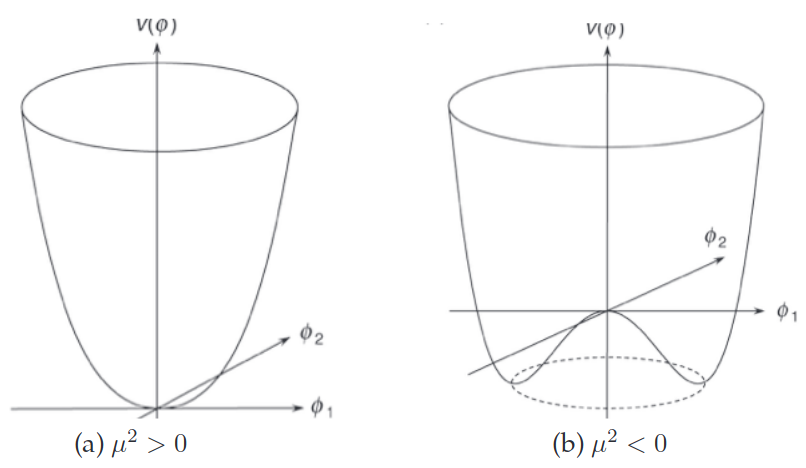
\includegraphics[width=0.8\textwidth]{Images/higgs_potential.png}
    \caption{Illustration of the form of the Higgs potential depending on the sign of $\mu^2$.}
    \label{fig:mexicanhat}
\end{figure}

The expected value of the field in the vacuum (vev) is therefore the minimum of this potential. For the Higgs field this value is

\begin{equation}
    \langle \phi \rangle_0 = \frac{1}{\sqrt{2}}\sqrt{\frac{\mu^2}{\lambda}} \equiv \frac{v}{\sqrt{2}} \mend
\end{equation}

Physically, this means that the vacuum correspond to a non-zero expectation value for the Higgs field, which causes the spontaneous symmetry breaking, leading to massive weak bosons.

Since the Lagrangian is gauge invariant, the Higgs field can be described from its minimum without loss of generality by applying a gauge transformation, which conserves the number of degrees of freedom. It is fitting to re-express the field using an exponential decomposition :

\begin{equation}
    \phi(x) = \frac{1}{\sqrt{2}}e^{e\tau_a \theta^a (x) / f} \begin{pmatrix} 0 \\ \rho(x) \end{pmatrix}
\end{equation}
where $\theta^a$(x) and $\rho(x)$ are real fields, $\tau_a$ corresponds to the generators of $SU(2)$ and f is a unit normalization constant. $\theta^a$ contains three of the four degrees of freedom of the Higgs doublet, while $\rho$ conserves the remaining one, as a sort of module of the field.\newline

By expanding the Higgs field in a particular set of coordinate, one can break the vacuum symmetry. To get the physical observables, the expansion will be made around the position of the minimum of the field $v$. The new real field $h$ is then defined by translation as

\begin{equation}
    h(x) \equiv \rho (x) - \langle \phi \rangle_0 = \rho(x) - v \mend
\end{equation}

However this minimum is degenerated, meaning there are an infinite number of points satisfying the condition. The symmetry will be broken by choosing one point and developing the Higgs field around it. The simplest choice is the unitary gauge, in which the degrees of freedom are minimized. In this case it means setting all $\theta^a$ to 0, which is analogous to setting $\phi_2 = \phi_3 = \phi_4$. The Higgs field then becomes

\begin{equation}
    \phi(x) = \frac{1}{\sqrt{2}} \begin{pmatrix} 0 \\ v + h(x) \end{pmatrix} \mend
    \label{eq:simphiggsfield}
\end{equation}

Developing the Higgs lagrangian from equation \ref{eq:higgs_lagr} using this Higgs field form gives

\begin{align}
    \Lagr_H = \frac{1}{2}(\partial_{\mu}h)(\partial^{\mu}h) + \frac{1}{2}(2\mu^2 )h^2 + \frac{1}{2} \big( \frac{g^{2}_w v^2}{4} (W_{\mu}^1 W^{1\mu} + W_{\mu}^2 W^{2\mu}) \\ + \frac{1}{8} v^2 (g_W W_{\mu}^3 - g_B B_{\mu})(g_W W^{3\mu} - g_B B^{\mu}) + \mathcal{O}(h^2) \msep
    \label{eq:hlagr}
\end{align}

where $\mathcal{O}(h^2)$ refers to higher orders of the lagrangian, which include the coupling with the vector bosons and the self-coupling of the Higgs boson.

To obtain the physical bosons, the fields have to be rewritten in such a way that their mass terms be independent. For that purpose, new fields $A_{\mu}$, $W_{\mu}$ and $Z_{\mu}$ are defined as

\begin{equation}
    W^{\pm}_\mu = \frac{1}{\sqrt{2}}(W_{\mu}^1 \mp iW_{\mu}^2) \msep
\end{equation}
\begin{equation}
    Z_{\mu} = \mathrm{cos}(\theta_{W})W^3_{\mu} - \mathrm{sin}(\theta_{W_{\mu}})B_{\mu} \msep
\end{equation}

\begin{equation}
    A_{\mu} = \mathrm{cos}(\theta_{W})B_{\mu} + \mathrm{sin}(\theta_{W})W_{\mu}^3 \msep
\end{equation}
where the parameter $\theta_W$ is the Weinberg angle \cite{GLASHOW1961579} defined from the ratio of the coupling constants

\begin{equation}
    \mathrm{tan} \theta_W \equiv \frac{g_B}{g_W} \mend
\end{equation}
The coupling constants are related to the electric charge as :

\begin{equation}
    \frac{g_W g_B}{\sqrt{g_{W}^2 + g^{2}_B}} \equiv e
\end{equation}

Equation \ref{eq:hlagr} then becomes :

\begin{align}
    \MoveEqLeft[3]
    \Lagr_H = \frac{1}{2}(\partial_{\mu}h)(\partial^{\mu}h) + \frac{1}{2}\underbrace{(2\mu^2 )}_{m_{H}^2}h^2 \\ {}& + \frac{1}{2} \underbrace{(\frac{g_{w}^2 v^2}{4})}_{m_{W^+}^2} W_{\mu}^+ W^{+\mu} + \frac{1}{2} \underbrace{(\frac{g_{w}^2 v^2}{4})}_{m_{W^-}^2} W_{\mu}^- W^{-\mu} \\ {}& + \frac{1}{2} \underbrace{(\frac{g_W^2 v^2}{4\mathrm{cos}\theta_W})}_{m_Z^2} Z_{\mu} Z^{\mu} + \underbrace{0}_{m_{\gamma}^2}\times A_{\mu}A^{\mu}
\end{align} 

where mass terms appear for the different bosons. As one degree of freedom of the Higgs field is used to build the physical scalar Higgs field, one of the generators remains unbroken, which gives a massless boson, the photon.

The theoretical masses of the gauge bosons, obtained from the Fermi constant($G_F$) and the EW coupling constants $f_W$ and $g_B$ were confirmed experimentally \cite{ARNISON1983103,BANNER1983476,1983398,BAGNAIA1983130,Group:2008ds}. But as the Higgs boson mass depends on a free parameter of the theory, $\mu^2$, it could only be determined experimentally. It was eventually measured at $m_H \sim 125\,{\mathrm{GeV}}$ \cite{Aad2016}.\newline

The Higgs field can also interact with fermions. This interaction between a scalar field ($\phi$) and a Dirac field ($\psi$), called a Yukawa interaction, is a way to introduce gauge-invariant mass terms for fermions in the lagrangian. Before SSB, the Yukawa lagrangian is expressed as 

\begin{equation}
    \Lagr_{Y} = -i\lambda_f \Bar{L} \phi R_f - i\lambda_f\Bar{R}_f \phi L = -i\lambda_f (\Bar{L}\phi R_f + \Bar{R}_f \phi L)
\end{equation}
where the $\lambda_f$ terms are the coupling constants of the Higgs fields to the respective fermion $R_f$.

If the symmetry of the Higgs scalar doublet is spontaneously broken in the form of Equation \ref{eq:simphiggsfield}, a mass term for the down-type component of the fermion doublet appears. This would work for the lepton sector, as the neutrino-type is considered to be massless in the SM lagrangian, but it fails for up-type quarks, which also require a mass.

But the Higgs field can be rewritten in the charge-conjugated of the $SU(2)$ framework:

\begin{equation}
    \phi^c \equiv i\sigma_2 \phi^* = \begin{pmatrix} \phi^{(0)*} \\ -\phi^{(-)} \end{pmatrix}  \xrightarrow{\text{SSB}} \frac{1}{\sqrt{2}}\begin{pmatrix} -(v+h(x)) \\ 0 \end{pmatrix} 
\end{equation}
where $\sigma_2$ is the second Pauli matrix, generator of $SU(2)$. The Higgs field in this form provides the symmetry-breaking term as the upper component, meaning it couples with up-type quarks to provide a mass term.

The Yukawa lagrangian becomes:

\begin{align}
    \MoveEqLeft[3]
    \Lagr_Y = -i\lambda_e (\Bar{\nu}\Bar{e})_L \phi e_R - i\lambda_d (\Bar{u}\Bar{d})_L \phi d_R - i\lambda_u (\Bar{u}\Bar{d})_L \phi^c u_R \\ ={}& -i\lambda_f (\Bar{L}\phi R_f + \Bar{R}\phi L) - i\lambda_f(\Bar{L}\phi^c R_f + \Bar{R}\phi^c L) \\ ={}& -i\lambda_f(\Bar{L}\phi R_f + \Bar{L}\phi^cR_f) + h.c.
\end{align}

After picking the gauge, by arranging the chiralities, the lagrangian simplifies to:

\begin{equation}
    \Lagr_Y = \frac{-\lambda_f (v+h)}{\sqrt{2}}(\Bar{\psi}_R\psi_L + \Bar{\psi}_L\psi_R)
\end{equation}
therefore the mass terms of the fermions are:

\begin{equation}
    m_f \equiv \lambda_f \frac{v}{\sqrt{2}}
\end{equation}

Hence the coupling of the Higgs to a fermion is proportional to its mass, making heavier fermions, such as $\tau$ leptons, having an enhanced coupling to the Higgs boson.

In conclusion, the overall SM lagrangian can be written by combining all terms as:

\begin{equation}
    \Lagr_SM = \underbrace{- \frac{1}{4} F_{\mu\nu}^a F^{\mu\nu}_a}_{Free bosons} + \underbrace{i\Bar{\psi}\slashed{D}\psi}_{Fermion term} +\underbrace{i\lambda_f(\Bar{L}\phi R_f + \Bar{L}\phi^cR_f) + h.c.}_{Yukawa interaction} + \underbrace{|D_{\mu}\phi|^2 - V(\phi)}_{Higgs mechanism}
\end{equation}
where:
\begin{align*}
    & F_{\mu\nu}^a F^{\mu\nu}_a \equiv G_{\mu\nu}^a G^{\mu\nu}_a + W_{\mu\nu}^a W^{\mu\nu}_a + B_{\mu\nu}^a B^{\mu\nu}_a \\
    & i\Bar{\psi}\slashed{D}\psi \equiv i\Bar{\psi}\gamma^{\mu} (\partial_{\mu} - g_s T_a G_{\mu}^a - g_W T_a W^{a}_{\mu} - g_B Y B_{\mu})  \psi \\
    & D_{\mu}\phi \equiv (\partial_{\mu} - ig_W T_a W_{\mu}^{a} - ig_B B_{\mu})\phi \\
    & V(\phi) \equiv \lambda(\phi^{\dagger}\phi)^2 - \mu^2 (\phi^{\dagger}\phi) &&
\end{align*}

and the experimental value of the nineteen free parameters of the SM are in Table \ref{tab:SMparams}.

\begin{table}[]
    \centering
    \caption{Experimental value of the 19 free parameters of the standard model.}
    \begin{tabular}{l c r c}
        \hline
        \textbf{Name} & \textbf{Symbol} & \textbf{Value} & \\
        \hline
        Up quark mass & $m_u$ & $2.2^{+0.6}_{-0.4}$ & MeV \\
        Charm quark mass & $m_c$ & $1.27 \pm 0.03$ & GeV \\
        Top quark mass & $m_t$ & $173.1\pm0.6$ & GeV \\
        Down quark mass & $m_d$ & $4.7^{+0.5}_{-0.4}$ & MeV \\
        Strange quark mass & $m_s$ & $96^{+8}_{-4}$ & MeV \\
        Bottom quark mass & $m_b$ & $4.18^{+0.04}_{-0.03}$ & GeV \\
        Electron mass & $m_e$ & $0.511\pm(0.31\times10^{-8})$ & MeV \\
        Muon mass & $m_{\mu}$ & $105.66\pm(0.24\times10^{-5})$ & MeV \\
        Tau mass & $m_{\tau}$ & $1776.86\pm0.12$ & MeV \\
        CKM I-II mixing angle & $\theta_{12}$ & $(13.01 \pm 0.03)$\degree & \\
        CKM II-III mixing angle & $\theta_{23}$ & $(2.35 \pm 0.09)$\degree & \\
        CKM I-III mixing angle & $\theta_{13}$ & $(0.20 \pm 0.04)$\degree & \\
        CKM CP-violating phase & $\delta_{\mathrm{CKM}}$ & $(70 \pm 3)$\degree & \\
        $U(1)_{Y}$ gauge coupling & $g_{B}$ & $0.34970 \pm 0.00019$ & \\
        $SU(2)_{L}$ gauge coupling & $g_{W}$ & $0.65295 \pm 0.00012$ & \\
        $SU(3)_{C}$ gauge coupling & $g_{s}$ & $0.1182 \pm 0.00012$ & \\
        QCD vacuum angle & \theta_{\mathrm{QCD}} & $< 10^{-10}$ & $\sim 0$ \\
        Higgs v.e.v. & $v$ & $246 \pm (6\times 10^{-5})$ & GeV \\
        Higgs boson mass & $m_H$ & $125.09 \pm 0.24$ & GeV 
    \end{tabular}
    \label{tab:SMparams}
\end{table}

\subsection{Issues of the Standard Model}
\label{sec:SM_limits}

While the SM is a huge breakthrough, it still provides an incomplete description of nature, as it lacks explanation for several phenomena. 

\paragraph{Gravity} The gravitational force has not been quantized yet, and therefore cannot be included in a QFT such as the SM. Indeed the connection between quantum physics and general relativity, which is by essence the theory of gravitation, has not been theorized. However, in an experimental particle physics context, gravitation is negligible. Indeed, no experiment within the field has been accurate enough to pinpoint the effect of gravity at a particle level.

\paragraph{Neutrino masses and right-handed neutrinos} Neutrinos do not interact with the Higgs boson, since they are massless fermions in the current SM lagrangian. However, experimental observations such as the neutrino oscillation \cite{PhysRevLett.81.1562,PhysRevLett.89.011301} prove that they are massive particles.

Another issue rises from the neutrinos being massive : the EWT is a chiral theory that violates parity maximally, and only left-handed neutrinos are required in its formulation. However, being indeed massive, their right-chirality particles must exist in nature although do not interact, and therefore cannot be included in the SM. Several hypothesis, as the seesaw mechanism \cite{PhysRevD.22.2227,PhysRevLett.60.1813,PhysRevD.23.165,PhysRevLett.44.912,GellMann:1980vs,MINKOWSKI1977421} have been proposed to describe these sterile neutrinos but these hypotheses are not supported by any experimental evidence.

\paragraph{Dark matter} Dark matter is postulated to be a type of matter which interacts gravitationally but not electromagnetically, as its presence can be inferred from the shape and rotation speed of galaxies, but does not give off or interacts with light. The SM does not account for a candidate for this dark matter.

\paragraph{Dark energy} Dark energy is also a postulate from astro-physics observations. Indeed, the measurements linked with of the expansion of the universe imply acceleration. The energy that would correspond to this phenomenon would account for $73\%$ of the energetic content of the universe. 

\paragraph{Anti-matter asymmetry} The Dirac equation predicts that each particle is created with an anti-matter partner with opposite quantum numbers. But the observed universe is mainly made up of regular matter, and even though EWT provides a CP-symmetry violating mechanism that can explain such asymmetry, the scale of the asymmetry does not match the effect of such phenomena alone.\newline

Although the SM lacks explanations for all these phenomena, it has provided extremely precise predictions. Therefore the SM can be considered as an effective theory, while a deeper more complete description of the subatomic world exists. Such theories are said to be beyond the standard model (BSM), with an example being the minimal supersymmetric extension of the standard model (MSSM).


\section{The Minimal Supersymetric extension of the Standard Model}
\label{sec:MSSM}

One of the promising BSM models is Supersummetry (SUSY) as it extends the symmetries of the standard models, solving many issues and providing a Dark Matter candidate. SUSY \cite{Martin:1997ns} introduces a new symmetry between fermions and bosons, making them effectively not independent objects but flavors of a more fundamental field. From this symmetry the existence of superpartners of each of the SM fermions and bosons is inferred. Each fermion therefore has a bosonic partner, called sfermion, which carries an integer spin. Conversely each boson has a fermionic partner called bosino, which carries a semi-integer spin. Both objects belong to a multiplet with the same quantum numbers except the spin.\newline

However, none of the superpartners have been observed so far, leading to the conclusion that this symmetry must be broken at the current energy scale. Indeed, the SUSY theory implies the addition of a big set of new, undiscovered, observable particles, along with more free parameters in the theoretical formulation, in particular the masses of the new particles.\newline

A consequence of the SUSY models could be the unification of the three forces of nature, namely electromagnetic, weak and strong interactions, into one, making such model a Grand Unified Theory (GUT). Indeed the unification of the weak and electromagnetic forces is already achieved in the SM with EWT, but the QCD and EW theories do not seem to converge. If SUSY interactions are added, the running couplings of the forces could be modified in such a way that they would converge at a large energy scale, thus providing a natural mechanism for a GUT.\newline

Since SUSY is a general framework which depends on many unknown parameters, it can be implemented in different forms. The simplest model that realizes SUSY while being compatible with the current observations is called the Minimal Supersymmetric Standard Model (MSSM). The aim is to add the minimal amount of new parameters, particles and interactions, while keeping all the current symmetries and observables of the SM. Table \ref{tab:superpartners} summarizes the symmetry between ordinary particles and their superpartners.

\begin{table}[]
    \centering
    \caption{Relations between the SM particles and their superpartners, before the EW symmetry-breaking, according to the MSSM. In the MSSM, the ordinary SM Higgs sector requires four additional Higgs bosons $H$, $A$ and $H^{\pm}$ in addition to the SM Higgs, called $h$ here.}
    \begin{tabular}{c c c c | c c c c}
        \hline
         \multicolumn{4}{c}{\textbf{SM particle} (R = +1)} & \multicolumn{4}{c}{\textbf{Superpartner} (R = -1)} \\
        Type & Spin & Particle & Symbol & Symbol & Particle & Spin & Type \\
        \hline
        \multirow{2}{*}{Fermions} & \multirow{2}{*}{1/2} & Quark & $\psi_f$ & $\Tilde{\psi}_f$ & Squark & \multirow{2}{*}{0} & \multirow{2}{*}{SFermions} \\
         & & Lepton & $\psi_l$ & $\Tilde{\psi}_l$ & Slepton & & \\
         \hline
         \multirow{5}{*}{Bosons} & \multirow{3}{*}{1} & Gluon & g & $\Tilde{g}$
   & Gluino & \multirow{5}{*}{1/2} & \multirow{5}{*}{Bosinos} \\
          & & W & $W^i$ & $\Tilde{W}$ & Wino & & \\
          & & B & B & $\Tilde{B}$ & Bino & & \\
          & \multirow{2}{*}{0} & \multirow{2}{*}{Higgs} & h, H, & $\Tilde{h}$, $\Tilde{H}$, & \multirow{2}{*}{Higgsinos} & & \\
          & & & $H^{\pm}$, A & $\Tilde{H}^{\pm}$, $\Tilde{A}$ & & & \\ 
          \hline
    \end{tabular}
    \label{tab:superpartners}
\end{table}

This approach would allow certain interactions which have not been observed in the SM. In particular, SUSY models could allow processes where the baryon ($B$) and Lepton($L$) numbers are not conserved, and by extension $B - L$ either. Since processes violating these numbers would make the proton unstable, which has not been observed, a new symmetry has to be added to the MSSM to suppress the $B-L$ violating process : the $R-parity$. The operator of said $R$-parity, which is discrete, is defined for each particle in an interaction as :

\begin{equation}
    P_R = (-1)^{3(B-L)-2s}
\end{equation}
where $s$ stands for the spin of the particle, $B$ and $L$ are the baryon and lepton number, respectively. The SM particles are defined as having $P_R = 1$ while superpartners have $P_R = -1$. To conserve $R$-parity the combined $P_R$ has to be positive. SUSY models conserving $R$-parity have an additional consequence : the lightest supersymmetric particle (LSP) is stable, thus chains of heavier SUSY particles end in the LSP. If the LSP is, in addition, electrically neutral, it would be a candidate for the composition of Dark Matter. Multiple searches looking for a LSP are being performed but no evidence of its existence has been observed so far.\newline

Adding a unique fermionic superpartner for the Higgs boson (named higgsino) has several implications. First, a chiral anomaly would appear, meaning the generation of low mass-states due to the non-conservation of a chiral current. These states have not been observed in the Higgs sector, so a mechanism to suppress such states must be present. Second, the suppression of the flavor-changing neutral currents, which are not observed in nature either, is not granted. Finally, the ratio between the neutral($G_n$) and charged ($G_c$) currents in the EWT could not be of the order of unity, in contradiction with observations. The simplest solution which avoid these issues, recovering the observations of the SM, is the addition of a second Higgs field doublet.

Mathematically the simplified Higgs potential can be written as \cite{Nagashima:2014tva}:

\begin{align}
    V(\phi_d , \phi_u) = & \mu^{2}_u (\phi^{\dagger}_u \phi_u) + \mu^{2}_u (\phi^{\dagger}_d \phi_d) - \mu^{4}(\epsilon_{ij}\phi^{i}_d \phi^{j}_u + h.c.) \\ & + \frac{g^{2}_W + g^{2}_B}{8}(\phi^{\dagger}_d \phi_d - \phi^{\dagger}_u \phi_u) + \frac{g^{2}_W}{2} | \phi^{\dagger}_d \phi_u |^2
\end{align}
where $\epsilon_{ij} = 0$ if $i = j$ and $\epsilon_{ji} = -\epsilon_{ij} = 1$.To ensure vacuum stability, the potential must be bound from below, meaning $\mu_{d}^2 + \mu_{u}^2 > 2\mu^2$. The requirement for the spontaneous symmetry breaking becomes $\mu^4 > \mu_{u}^2 \mu_{d}^2$, and the symmetry is spontaneously broken by the choice of the non-zero vacuum at:

\begin{align}
    \langle \phi_d \rangle = \frac{1}{\sqrt{2}} \begin{pmatrix} 0 \\ \nu_d \end{pmatrix} \\
    \langle \phi_d \rangle = \frac{1}{\sqrt{2}} \begin{pmatrix} \nu_u \\ 0 \end{pmatrix} \mend
\end{align}
The vacuum expectation value of the SM , $\nu$ is recovered by
\begin{equation}
    \nu^2 \equiv \nu_{d}^2 + \nu_{u}^2 \mend
\end{equation}
A useful parameter is $\beta$ defined as 
\begin{equation}
    \mathrm{tan} \beta \equiv \frac{\nu_u}{\nu_d} \mend
\end{equation}
The masses of the $W^{\pm}$ and $Z$ bosons are now defined as 
\begin{align}
    m_W \equiv \frac{v.g_W}{2} \\
    m_Z \equiv \frac{\mu_{d}^2 \mu_{u}^2 \times \mathrm{tan}^2 \beta}{\mathrm{tan}^2 \beta - 1} \mend
\end{align}

The Yukawa couplings of the different Higgs bosons to the quarks are also modified with respect to the SM. They can be expressed as a correction of the coupling of the SM boson, depending on $tan \beta$ and a second angle $\alpha$ defined as 

\begin{equation}
    \mathrm{tan} 2\alpha \equiv \frac{m_{A}^2 + m_{Z}^2}{m_{A}^2 - m_{Z}^2} \mathrm{tan}2\beta \mend
\end{equation}

The Yukawa couplings expressed in terms of the $\alpha$ and $\beta$ parameters can be found in table \ref{tab:yukawaMSSM}. Measurements of such couplings could be very powerful to discriminate between SM and MSSM.

\begin{table}[]
    \centering
    \caption{Relation of the Yukawa coupling parameters ($\lambda_ii$) with respect to the SM coupling ($\lambda_{SM}$) for the neutral MSSM Higgs bosons ($h$, $H$ and $A$) to the vector bosons ($\lambda_{VV}$), and to the different fermions, split in $u$-type (only quarks, $\lambda_{uu}$) and $d$-type (quarks and electron type $\lambda_{dd,ll}$) as a function of the angles $\alpha$ and $\beta$.}
    \begin{tabular}{c c c c}
        $\lambda_{ij}$ / $\lambda_{SM}$ & $\lambda_{VV}$ & $\lambda_{uu}$ & $\lambda_{dd,ll}$ \\
        \hline
        h & $\mathrm{sin}(\beta - \alpha)$ & $\mathrm{cos}\alpha/sin_\beta$ & $-\mathrm{sin}\alpha / cos\beta$ \\
        H & $\mathrm{cos(\beta - \alpha)}$ & $\mathrm{sin\alpha / sin\beta}$ & $\mathrm{cos\alpha / cos \beta}$ \\
        A & 0 & $\mathrm{cot\beta}$ & $\mathrm{tan\beta}$ \\
        \hline
    \end{tabular}
    \label{tab:yukawaMSSM}
\end{table}

The masses of the five Higgs bosons at tree level is then :

\begin{align}
    m_{A}^2 &= \frac{2\mu^2}{sin 2\beta} \\
    m_{H^{\pm}}^2 &= m_{A}^2 + m_{W}^2 \\
    m_{H,h}^2 &= \frac{1}{2} \big( m_A^2 + m_Z^2 \pm \sqrt{(m_A^2 + m_Z^2)^2 - 4m_Z^2 m_A^2 cos^2 2\beta} \big)
\end{align}

Indeed, at lowest order, the masses of the Higgs bosons depend on two free unknown parameters, which are conventionally chosen to be $tan \beta$ and $m_A$. However when higher-order corrections are included, several additional parameters such as the stop (top quark superpartner) mixing parameter :

\begin{equation}
    X_t \equiv A_t - \mu cot\beta
\end{equation}
which depends on the soft SUSY-breaking Higgs-stop coupling $A_t$. Another such parameter is the average scale of SUSY, defined as the average scale of the stop masses as

\begin{equation}
    m_{SUSY} \equiv \sqrt{m_{\Tilde{t_1}}m_{\Tilde{t_2}}} \mend
\end{equation}

Indeed, at higher orders the corrections on the Higgs mass becomes \cite{Nagashima:2014tva}

\begin{equation}
    \delta m_h^2 \approx \frac{3 m_t^4}{2\pi^2 v^2} \Big[ ln\frac{m_{SUSY}^2}{m_t^2} + \frac{X_t^2}{m_{SUSY}^2} \big( 1 - \frac{X_t^2}{12 m_{SUSY}^2} \big) \Big] \mend
\end{equation}

As a huge number of free parameters is impractical for experimental tests, a common procedure is to set high-order parameters to a particular value, aiming to focus on specific MSSM phenomenologies, called scenarios, and then set experimental limits on the $tan \beta$ vs $m_A$ parameters. Such scenarios  are detailed in section \ref{sec:pheno}.

The search for the additional neutral heavy Higgs boson of the MSSM is one of the goal of this thesis, as detailed in chapter \ref{sec:Analysis}. This search is done in several MSSM scenarios, aiming for topologies where the differences with respect to the SM is enhanced. 

\section{Phenomenology of MSSM Higgs bosons production and decay into $\tau\tau$ in $pp$ collisions at the LHC}
\label{sec:pheno}

In order to challenge not only the SM but also any BSM theories like the MSSM, many experiments have been designed, either to make indirect measurements of parameters, or to directly detect new particles by allowing their creation and detecting their decay products. The Large Hadron Collider was designed with both in mind. Indeed the LHC accelerates beams of protons to achieve the necessary energy in the center of mass to generate processes of interest. When two protons collide, most cases are elastic scatters due to the repulsion of their electric charge. But in some cases the interaction is inelastic, resulting in the production of new particles. Protons are hadrons, composite particles formed by three valence quarks, namely $uud$, that are bound together by a continuous exchange of gluons. Within the proton, gluons are transformed continuously in pairs of quark-antiquark, which forms the sea of quarks.

The main collision, called event, comes from the hard scattering of the protons at high energy, and can be described using a perturbative approximation of QCD, assuming asymptotic freedom. However, the collisions are dominated by the soft scattering, radiation of low energy interactions. The estimation of such processes cannot be done through perturbative QCD, and is therefore parametrized from data.

The elements that are effectively taking part of the collision, either quarks (valence or from the sea) or gluons,  are called partons. Since they are bound within the proton, they carry part of its energy in a dynamic way. Therefore the partons carry a fraction of the energy carried by the proton as a whole, meaning the energy available at the collision is a spectrum upperly bounded by the energy given to both protons. Several different probability distributions, called Parton Distribution Functions (PDFs) are used to estimate this energy distribution. Different PDF schemes, such as CTEQ \cite{Pumplin:2002vw}, MSTW \cite{Martin:2009iq} and NNPDF \cite{Ball:2008by} have been developed and tested at different energy regimes.

The cross-section of the pp collisions, $\sigma(pp\rightarrow X)$ is given by the QCD factorization theorem \cite{Butterworth:2012fj}:

\begin{equation}
    \sigma(pp\rightarrow X) = \sum_{i,j} \int \int f_i (x_1 , \mu_F^2 )f_j (x_2 , \mu_F^2 ) \hat{\sigma}_{ij \rightarrow X} (s x_1 x_2 , \mu_R^2 , \mu_F^2 ) dx_1 dx_2 
\end{equation}
where $x_1$ and $x_2$ variables are the fraction of the total momentum that the partons $i,j$ carry, providing an effective center-of-mass energy of $\hat{s} = sx_1 x_2$ , and the variables $\mu_R^2$ and $\mu_F^2$ are the renormalization and factorization factors respectively, which are obtained by truncating the strong coupling constant. Finally, the variables $f_i$ and $f_j$ are the parton densities, obtained from PDFs.

The partial cross-section $\hat{\sigma}_{ij \rightarrow X}$ can be computed using the perturbative method, up to Leading Order (LO), or adding further corrections to next orders, (NLO, NNLO,...). However, the physical process does not end here: the partons involved in the collision can irradiate soft-gluons (parton shower) which later will hadronize, forming a cascade of particles. An accurate theoretical modeling of these effects is not possible and thus, their simulation is constrained using experimental data.

On top of all this happening when a collision happens, several other interactions can occur simultaneously to the main collision event, due to the interactions of either other protons or from the remainder of the partons from the main event. these are called pile-up and underlying event, respectively.

\subsection{Higgs boson production}

At the LHC, neutral Higgs bosons can be produced in several different processes, which have been measured with great accuracy for the SM Higgs boson \cite{Dittmaier:1318996}. The cross-section of the SM Higgs boson production modes as a function of center-of-mass energy is shown in figure \ref{fig:higgscrosssec}.

\begin{figure}
    \centering
    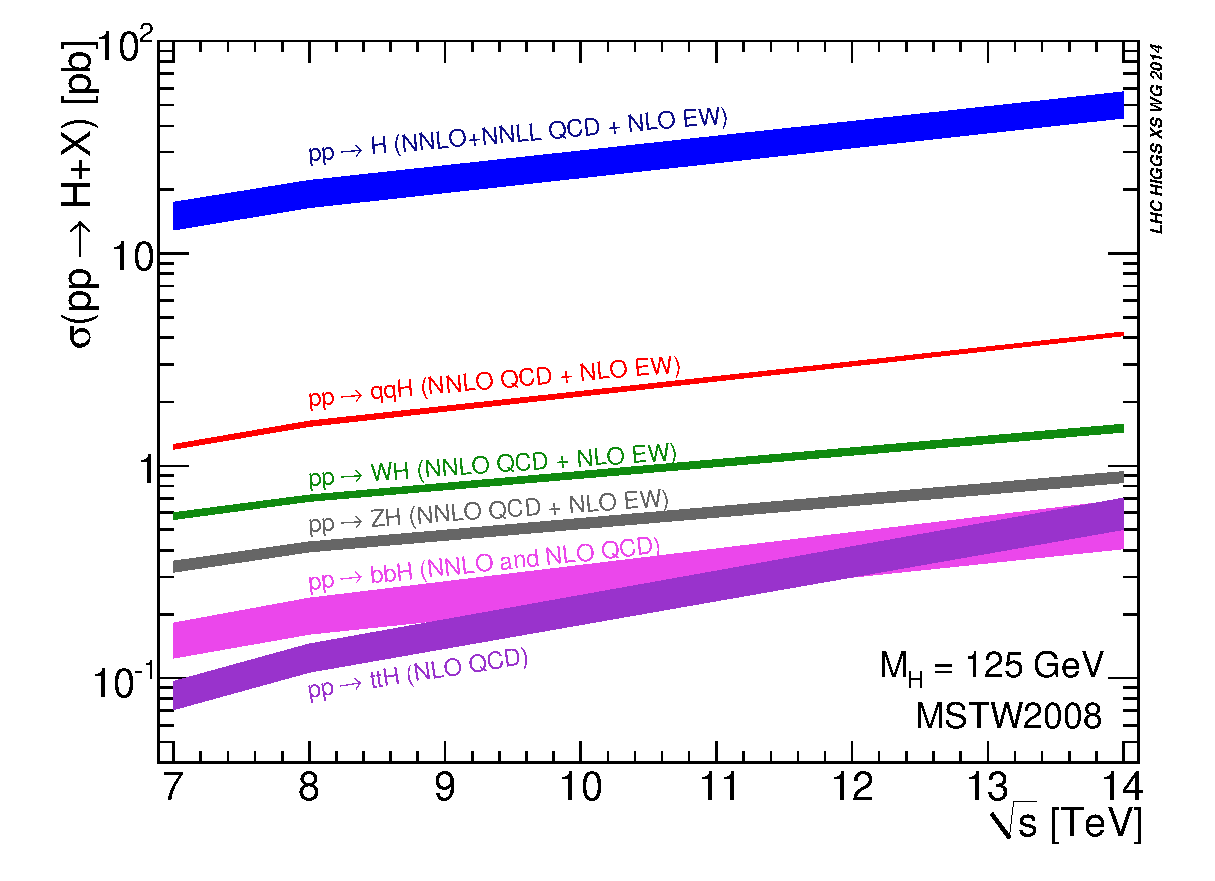
\includegraphics[width=0.7\textwidth]{Images/xsec.eps}
    \caption{Cross-sections for different Higgs boson production processes as a function of center of mass energies.}
    \label{fig:higgscrosssec}
\end{figure}

The dominant Higgs production process at the LHC is the gluon fusion, labeled ggH (Figure \ref{fig:ggh}). This interaction is mediated by a loop of quarks. Since the Yukawa coupling of the Higgs boson depends on the mass of the fermion, the top quark dominates this process. The ggH process is most abundant production mode, with up to $85\%$ of SM Higgs bosons production.


\begin{figure}
    \centering
    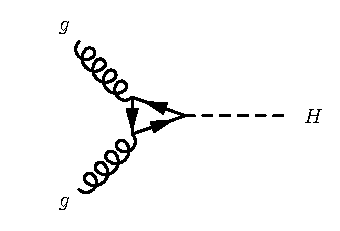
\includegraphics[width=0.4\textwidth]{Images/ggh.pdf}
    \caption{Feynman diagram for the gluon fusion process ($ggh$) at lowest order.}
    \label{fig:ggh}
\end{figure}


The second most abundant production mode at the LHC is the vector boson fusion \cite{PhysRevD.85.035002}, abbreviated as VBF (Figure \ref{fig:vbf}). This process consists of two quarks directly or indirectly producing two vector bosons ($W^{\pm}$ or $Z$) that fuse into a Higgs boson. Despite having a cross-section ten times lower than ggH at LHC, this process is particularly recognizable thanks to the behaviour of the two outgoing quarks, which hadronize giving two observable energetic jets back-to-back in the Higgs reference frame. The current computation of the cross-section includes NNLO QCD corrections and NLO EW corrections \cite{deFlorian:2227475}.


\begin{figure}
\centering
\begin{subfigure}[b]{0.5\textwidth}
  \centering
  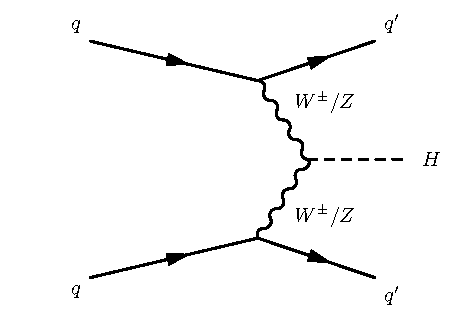
\includegraphics[width=\textwidth]{Images/VBF1.pdf}
  \caption{\label{fig:vbf1}}
\end{subfigure}%
\begin{subfigure}[b]{0.5\textwidth}
  \centering
  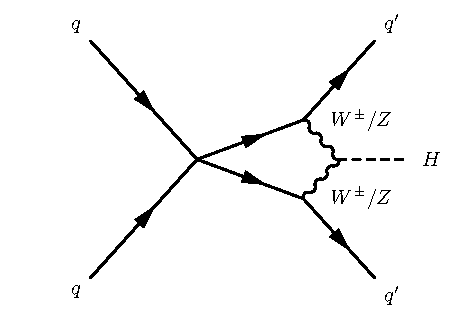
\includegraphics[width=\textwidth]{Images/VBF2.pdf}
  \caption{\label{fig:vbf2}}
\end{subfigure}
\caption{Feynman diagrams for the Vector Boson Fusion process of a Higgs boson with two jets at leading order for the $t$ (\subref{fig:vbf1}) and $u$ (\subref{fig:vbf2}) channels.}
\label{fig:vbf}
\end{figure}


Another process is the production of a Higgs boson in association with a vector boson, VH (Figure \ref{fig:vh}), also called Higgs-strahlung. In this process, the quark-antiquark pair collisions give rise to an energetic vector boson ($W^{\pm}$ or $Z$), which then radiates a Higgs boson. The cross-sections are computed up to NNLO for the QCD corrections plus NLO EW corrections \cite{deFlorian:2227475}.


\begin{figure}
\centering
\begin{subfigure}[b]{0.3\textwidth}
  \centering
  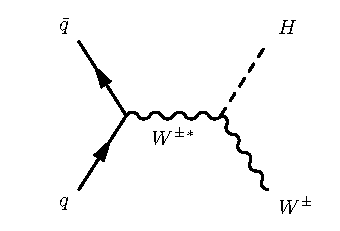
\includegraphics[width=\textwidth]{Images/VH1.pdf}
  \caption{\label{fig:vh1}}
\end{subfigure}%
\begin{subfigure}[b]{0.3\textwidth}
  \centering
  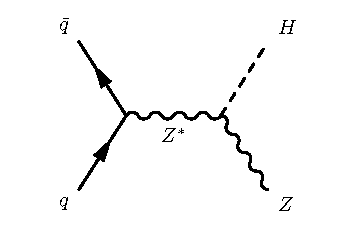
\includegraphics[width=\textwidth]{Images/VH2.pdf}
  \caption{\label{fig:vh2}}
\end{subfigure}%
\begin{subfigure}[b]{0.3\textwidth}
  \centering
  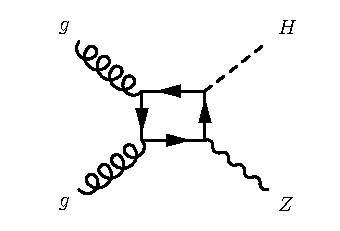
\includegraphics[width=\textwidth]{Images/VH3.pdf}
  \caption{\label{fig:vh3}}
\end{subfigure}
\caption{Feynman diagrams for the vector boson associated production process (VH) at leading order for (\subref{fig:vh1}) the W boson and (\subref{fig:vh2}) the Z boson. Last diagram (\subref{fig:vh3}) corresponds to a gluon fusion via top quark loop which contributes to the ZH mode.}
\label{fig:vh}
\end{figure}


Last but not least, another production process is the associated production with heavy fermions, namely top quarks ($\mathrm{t\Bar{t}H}$) and bottom quarks ($\mathrm{b\Bar{b}H}$), the latter shown in Figure \ref{fig:bbh}. Even though these modes are not significant in SM Higgs boson production at the LHC, the MSSM takes advantage of the enhanced coupling of the $b$-quark to the Higgs bosons for large $\mathrm{tan} \beta$ values. In such cases this mode becomes a significant or even dominant source of Higgs bosons. The cross-section for the $\mathrm{b\Bar{b}H}$ modes are computed at NLO for the 4-flavor scheme, in which it is assumed that the only 4 lightest quarks being available in the proton, and NNLO for the 5-flavor scheme \cite{deFlorian:2227475}.


\begin{figure}
\centering
\begin{subfigure}[b]{0.22\textwidth}
  \centering
  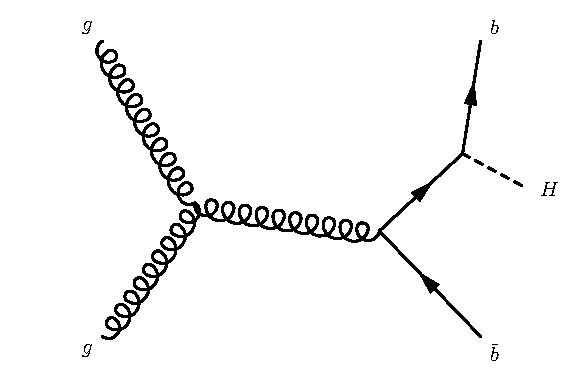
\includegraphics[width=\textwidth]{Images/bbh1.pdf}
  \caption{\label{fig:bbh1}}
\end{subfigure}%
\begin{subfigure}[b]{0.22\textwidth}
  \centering
  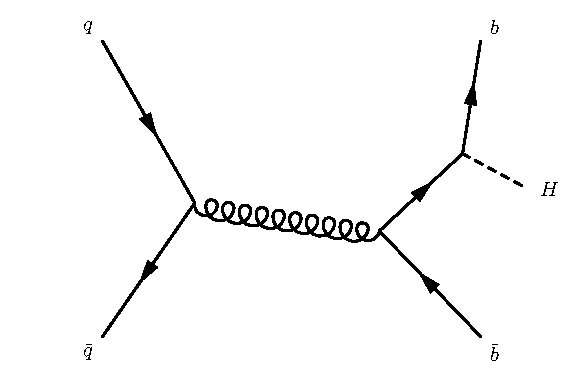
\includegraphics[width=\textwidth]{Images/bbh2.pdf}
  \caption{\label{fig:bbh2}}
\end{subfigure}%
\begin{subfigure}[b]{0.22\textwidth}
  \centering
  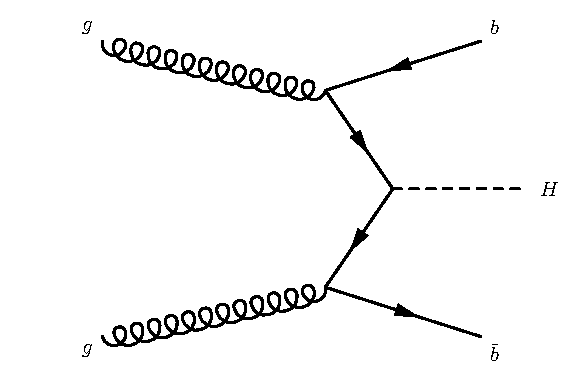
\includegraphics[width=\textwidth]{Images/bbh3.pdf}
  \caption{\label{fig:bbh3}}
\end{subfigure}
\begin{subfigure}[b]{0.22\textwidth}
  \centering
  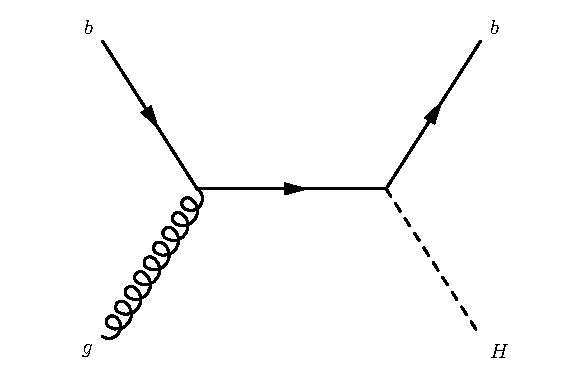
\includegraphics[width=\textwidth]{Images/bbh4.pdf}
  \caption{\label{fig:bbh4}}
\end{subfigure}%
\caption{Feynman diagrams for the $b$-associated production process at leading order in the four-flavour scheme (\subref{fig:bbh1},\subref{fig:bbh2},\subref{fig:bbh3}) and the five-flavour scheme (\subref{fig:bbh4}).}
\label{fig:bbh}
\end{figure}

\subsection{Higgs bosons decay}

Higgs bosons have a very short life time. For example, the SM Higgs boson has a life time of $\sim 10^{-22} \, \mathrm{s}$ \cite{pdg2016}. Hence direct observations are unfeasible and the searches have to focus on the signatures of their decays. Each of the decay modes have a different topology as well as different branching ratios (BR). 

The MSSM introduces a second Higgs doublet because of theoretical requirements covered in section \ref{sec:MSSM}, leading to five observable Higgs boson, namely $h$, $H$, $A$ and $H^{\pm}$. The most common interpretation of the discovered Higgs boson at $\sim 125\, \mathrm{GeV}$ in the MSSM context is to assume that it holds the role of the lightest boson $h$. This thesis will rely on this interpretation to look for other neutral Higgs bosons with masses larger than $m_h = 125 \pm 3 \, \mathrm{GeV}$. The MSSM modifies the relations of the masses and couplings of the Higgs particles with respect to the SM. At tree level, the correction to the masses can be written to depend uniquely on the $m_A$ and $\mathrm{tan} \beta$ parameters, while the corrections to the Yukawa couplings of the heavy neutral Higgs bosons to down type fermions can be written in terms of the angles $\alpha$ and $\beta$ as

\begin{equation}
    \lambda(H \rightarrow bb, \tau\tau) \propto \frac{\mathrm{cos} \alpha}{\mathrm{cos} \beta} = \frac{\mathrm{cos} \alpha}{\mathrm{sin} \beta} \mathrm{tan} \beta
\end{equation}
\begin{equation}
    \lambda(A \rightarrow bb, \tau\tau) \propto \mathrm{tan} \beta \mend
\end{equation}
Therefore, the coupling of both heavy neutral Higgs bosons are proportional to the value of the free parameter $\mathrm{tan} \beta$. Therefore, for large values of $\mathrm{tan} \beta$ the coupling of these Higgs bosons to $d$-type fermions, such as the $b$ quark and the $\tau$ lepton is enhanced with respect to the SM. This difference can not only be used to discriminate between SM and MSSM, but also leads to new ways of detecting Higgs decays that were not favored in the SM. Large $tan \beta$ values would lead to an enhancement of the $H \rightarrow \tau\tau$ and $H \rightarrow bb$ branching ratios, and of the $\mathrm{b\Bar{b}H}$ production mode cross section \ref{fig:bbh}.

A large $\mathrm{tan} \beta$ would also affect the $\mathrm{g\Bar{g}H}$ mode, as the Higgs boson production in this mode happens through a quark loop. Contrarily to the SM, where the top loop dominates because of its mass, in the MSSM, a large value $\mathrm{tan} \beta$ would enhance $b$-quark loops, which could even dominate over $t$-loops.\newline


This thesis searches for a massive neutral Higgs boson decaying to a pair of $\tau$ leptons, denoted as $H, A \rightarrow \tau\tau$ channel, whose Feynman diagram is shown in Figure \ref{fig:htt}. The $H,A \rightarrow \tau\tau$ is a very sensitive fermionic channel despite its relatively low branching ratio because its final state provides a clear signature (high energetic $\tau$ leptons), while the more abundant $H,A \rightarrow bb$ channel suffers from significant backgrounds at the LHC.

\begin{figure}
    \centering
    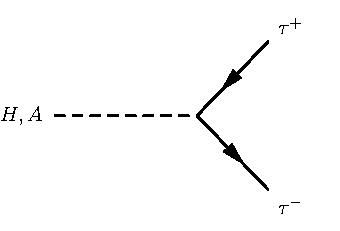
\includegraphics[width=0.5\textwidth]{Images/htt.pdf}
    \caption{Feynman diagrams for the $H,A \rightarrow \tau\tau$ decay at tree level.}
    \label{fig:htt}
\end{figure}

\subsection{The $\tau$ lepton}
\label{sec:tau_lepton}
The $\tau$ lepton is an unstable particle with a mean life of $\sim 10^{-13} s$ \cite{pdg2016} and therefore, a decay length of $87.03\, \mathrm{\mu m}$. Its decaying vertex is therefore usually close to the production vertex. The $\tau$ decays via the electroweak interaction, involving a virtual $W$, as illustrated in figure \ref{fig:tau_decay}.

\begin{figure}
    \centering
    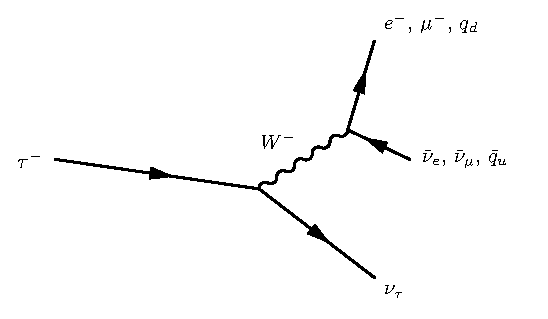
\includegraphics[width=0.6\textwidth]{Images/taudecay.pdf}
    \caption{Feynman diagram for the decay of the of a $\tau^-$ particle, mediated by a $W^-$ boson at tree level.}
    \label{fig:tau_decay}
\end{figure}

Leptonic $\tau$ decays produce an electron or a muon, and two neutrinos. Hadronic $\tau$ decays, denoted \tauh, lead to a single neutrino and a quark-antiquark pair. This decay leads to observed final states of mainly either 1 or 3 charged hadrons, and potentially several \pizero which decay to photons. On the other hand a $\tau$ lepton can lead to a an electron or muon, and neutrinos in the final states. All the important $\tau$ decays and their branching fractions are detailed in Table \ref{tab:tau_decay_products}. 

these different decays can lead many different final states of $H,A \rightarrow \tau\tau$ events. This thesis will focus on the fully hadronic channel, denoted $\tau_h \tau_h$.


\begin{table}[]
    \centering
    \caption{Branching fractions of the main (negative) $\tau$ decay modes. The generic symbol $h^-$ represents a charged hadron, pion or kaon. In some cases, the decay products arise from an intermediate mesonic resonance.}
    \begin{tabular}{l c c}
        \hline
         Decay mode & Meson resonance & Branching fraction [\%] \\
         \hline
         $\tau^- \rightarrow e^- \Bar{\nu_e} \nu_\tau$ & & 17.8 \\
         $\tau^- \rightarrow \mu^- \Bar{\nu_\mu} \nu_\tau$ & & 17.4 \\
         & &  \\
         $\tau^- \rightarrow h^- \nu_\tau$ & & 11.5 \\
         $\tau^- \rightarrow h^- \pizero \nu_\tau$ & $\rho$(770) & 26.0 \\
         $\tau^- \rightarrow h^- \pizero \pizero \nu_\tau$ & $a_1(1260)$ & 10.8 \\
         $\tau^- \rightarrow h^- h^+ h^- \nu_\tau$ & $a_1(1260)$ & 9.8 \\
         $\tau^- \rightarrow h^- h^+ h^- \pizero \nu_\tau$ & & 4.8 \\
         & &  \\
         Other modes with hadrons & & 1.8 \\
         All modes containing hadrons & & 64.8 \\
         \hline
    \end{tabular}
    \label{tab:tau_decay_products}
\end{table}
